\documentclass[a4paper,12 pt]{article}

%% Language and font encodings
\usepackage[spanish,es-tabla]{babel}
\usepackage[utf8]{inputenc}
\usepackage[T1]{fontenc}
\usepackage{cite}
\usepackage{amsmath, amsthm, amssymb, amsfonts} 
\usepackage[mathscr]{eucal}
\usepackage{ulem} % subrayar, tachar
\usepackage{hyperref} % para el url
\usepackage{multirow, array} % para las tablas
\usepackage{float} % para tablas [H]
\usepackage{graphicx} % graficos
\usepackage{titlesec} %subsubsubsection
\usepackage[usenames]{color} %palabras con color
\usepackage{lscape} % texto horizontal
\usepackage{pdflscape} % hoja horizontal
\usepackage{booktabs} %tabla con puntos

\newcolumntype{P}[1]{>{\centering\arraybackslash}p{#1}}
\newcolumntype{M}[1]{>{\centering\arraybackslash}m{#1}}
\newcolumntype{L}[1]{>{\raggedleft\arraybackslash}p{#1}}
\newcolumntype{R}[1]{>{\raggedright\arraybackslash}p{#1}}
  
%counter
\newcounter{mycounter} % create a new counter, called 'mycounter'
% default def'n of '\themycounter' is '\arabic{mycounter}'

%% command to increment 'mycounter' by 1 and to display its value:
\newcommand\showmycounter{\stepcounter{mycounter}\themycounter}

\usepackage{lipsum}
\newcommand\showlips{\stepcounter{mycounter}\lipsum[\value{mycounter}]}


%% Sets page size and margins
\usepackage[a4paper,top=2.5cm,bottom=2.5cm,left=2.5cm,right=2.5cm,marginparwidth= 1.5cm]{geometry}
  
\title{\LARGE \textbf{\\[0.5cm] Ingenio\\[2.5cm]}}

% Chicos, porfavor incluyan sus nombres en orden alfabetico
\author{\textbf{Grupo 7}\\[0.5cm]
        Valeria Huepa Ducuara\\
        Juan José Peña Becerra\\
        Carlos Daniel Rincón Mora\\
        Guiselle Tatiana Zambrano Penagos\\[2.5cm]
        Sebastian David Moreno Bernal\\[2.5cm]}
\date{}

\begin{document}

\newpage

\begin{figure}
    \centering
    
\includegraphics[width=0.57\textwidth]{images/escudoUN.png}
\end{figure}
\maketitle 
\thispagestyle{empty}

\begin{center}
    \small Universidad Nacional de Colombia\\
    Facultad de Ingeniería\\
    Departamento de Ingeniería de Sistemas e Industrial\\
    Ingeniería de Sistemas\\
    Ingeniería de Software II\\
    Bogotá, Colombia\\
    2020
\end{center}
\newpage
\tableofcontents % indice de contenidos}
\thispagestyle{empty}

\newpage
\setcounter{page}{1}
\pagestyle{plain}

\section{Descripción General}


\subsection{Descripción del Problema}

Dada la existencia de una necesidad de tener una plataforma online, adicionalmente no
existen muchos canales de información para personas interesadas en el campo de la
Ingeniería que quieran mantenerse informadas diariamente por medio de informes,
artículos y noticias de parte de una fuente confiable y en constante actualización,
esto es porque los canales existentes no se mantienen en continuo mantenimiento o no
son de agrado para el público en mención. Así mismo, hoy en día circulan noticias
falsas por redes sociales, y en otros medios de comunicación quitando la certeza y
veracidad de la información. Se desea una plataforma más personal, en donde las
personas del campo de la Ingeniería pueden conocerse e interactuar entre ellas, para
obtener conocimiento en diversas áreas en común de interés para cada uno, además de
comentar a los demás usuarios su opinión de cierto tema.\\

\subsection{Descripción del Producto}

El software a realizar pretende tener un vínculo con el público interesado en temas
actuales de Ingeniería (Stakeholders), y desea brindarle información de primera mano,
así como artículos (científicos, de opinión y periodísticos ) de gran interés para el
mundo actual, con autores de renombre en la industria de Ingeniería. Así mismo, podrán
registrarse para recibir notificaciones cada que algún artículo de su posible interés
sea publicado. Recibirán notificaciones de sus autores preferidos, para mantenerse
actualizados con el trabajo de reconocidos ingenieros.\\

Se desea realizar una plataforma más personal, que las que existen actualmente, en la
cual los usuarios puedan conocer a otras personas con intereses similares en el campo
de la Ingeniería, además de conocer, seguir y comentar el trabajo de otros ingenieros.
El registro como usuario es de carácter público, mientras que para que para ser autor y
poder realizar una publicación, esté debe ser aprobado por el administrador,
demostrando conocimiento en un área de interés, presentado comprobantes de estudios y
experiencia académica o laboral.\\

La plataforma cuenta con diferentes foros, en los cuales los usuarios podrán dar su
opinión de forma libre, siempre y cuando sean respetuosos con los demás usuarios y
autores, en caso contrario su cuenta podría ser vetada o eliminada de la plataforma.

% arreglar: Mejorar la descripción de los roles
\subsection{Descripción de los Roles de Usuario}

\begin{itemize}
    \item \textbf{Administrador:} Individuo que posee permisos especiales que le 
    permiten otorgar o despojar el rol de autor para los usuarios, este tendrá que
    verificar que el usuario que desee publicar contenido en la plataforma posea
    comprobantes que respalden su experiencia académica y laboral sobre uno o varios
    temas relacionados con la ingeniería, también será el responsable de atender las
    diferentes denuncias realizadas por los usuarios y determinar si es pertinente o 
    no vetar o eliminar al usuario denunciado.
    
    \item \textbf{Autor:} Individuo que posee el rol de usuario y autor, este puede 
    publicar contenido relacionado con la ingeniería en la plataforma e interactuar
    con los demás usuarios, para publicar información este puede hacerlo en formato
    PDF, JPG o PNG, podrá agregar archivos de opinión, investigación y noticias
    clasificándolos en una o mas categorías (computación, electrónica y robótica)
    y presentar esta información por medio de infografías, o texto plano.
    
    \item \textbf{Usuario:} Es el rol que tendrán todos los individuos que se
    registren en la plataforma, este podrá suscribirse a una o más categorías lo que
    le permitirá tener una sección de cada una en la pantalla de inicio, con los
    diferentes archivos pertenecientes a esta. Este también podrá seguir a autores y
    otros usuarios y recibir notificaciones cada vez que estos publiquen archivos de
    información o realicen comentarios en los foros. Este usuario podrá acceder a la
    información de la plataforma por medio de un buscador general (filtrando por
    palabras clave) o especializada (fecha de publicación, autor, categoría y tipo).
    
    \item \textbf{Visitante:} Este podrá ver la pagina principal de noticias y
    acceder al buscador general (filtrando por palabras clave), podrá ver las
    diferentes categorías y acceder a los artículos e infografías, más no podrá
    suscribirse a ninguna categoría, seguir autores o usuarios ni comentar en ningún
    foro. Si este desea acceder a más funcionalidades, tendrá que registrarse a la
    plataforma.
\end{itemize}{}

\section{Descripción del Equipo y Metodología de Desarrollo}

La metodología a seguir en este proyecto es Scrum, siguiendo todas las etapas y
características de la metodología mencionada. El manejo del código de software se
manejará por medio de un sistema de control de versiones central, usando las
herramientas Git y GitHub por parte de cada uno de los desarrolladores. \\

Para el correcto avance del proyecto se realizarán entregas parciales con análisis de
cada aspecto de este. Las fechas de los avances del proyecto serán de la siguiente
manera:

\begin{itemize}
    \item \textbf{Iteración 0:} Marzo 24 del 2020
    \item \textbf{Iteración 1:} Abril 14 del 2020
    \item \textbf{Iteración 2:} Mayo 5 del 2020
    \item \textbf{Iteración 3:} Mayo 26 del 2020
    \item \textbf{Iteración 4:} Junio 16 del 2020
    \item \textbf{Iteración Final:} Junio 23 del 2020
\end{itemize}{}

\subsection{Roles del equipo}

La forma en la que se trabajará durante el desarrollo del software será en equipos de 2
personas, donde uno de ellos trabajará en el front-end y otro en el back-end, los
equipos serán redefinidos en cada iteración y estos mantendrán comunicación diaria,
mientras que los reportes de avances por equipo serán realizados 2 veces por semana,
donde todos los desarrolladores estarán presentes.

\begin{table}[H]
    \centering
    \small{
    \begin{tabular}{|c|c|}
        \hline
        \textbf{Rol}   &   \textbf{Nombre}  \\ 
        \hline
        Product Owner   &   Sebastian David Moreno Bernal\\
        \hline
        Scrum Master   &   Guiselle Tatiana Zambrano Penagos\\
        \hline
        \multirow{2}{2cm}{Front End}    &   Valeria Huepa Ducuara\\
            &   Carlos Daniel Rincón Mora\\
        \hline
        \multirow{2}{2cm}{Back End}    &   Juan José Peña Becerra\\
            &   Guiselle Tatiana Zambrano Penagos\\
        \hline
         
    \end{tabular}
    \caption{Roles del equipo}}
    \label{T00}
\end{table}{}

\subsection{Recursos del equipo}

\begin{table}[H]
    \centering
    \small{
    \begin{tabular}{|M{2cm}|M{1.5cm}|M{3cm}|M{3cm}|M{1.5cm}|M{2cm}|}
        \hline
        \textbf{Nombre}    &\textbf{Marca}     &\textbf{Sistema Operativo} 
        &\textbf{Procesador}   &\textbf{RAM}   &\textbf{Capacidad}\\
        \hline
        Valeria Huepa                       &Asus   &Windows 10 Home x64 
        & Intel(R) Core(TM) i5-4210U CPU    &12GB   &HDD 240GB \\
        \hline
        Juan Peña                           &Asus   &Windows 10 Home x64
        &Intel(R) Core(TM) i5-6198DU CPU @ 2.30 GHz &8GB    &HDD 240GB\\
        \hline
        Carlos Rincón                       &Asus   &Windows 10 Home x64
        &Intel(R) Core(TM) i7-3537U CPU @ 2.00GHz   &8GB    &SSD 128GB\\
        \hline
        Tatiana Zambrano                    &Lenovo &Kali Linux x64
        &AMD A8 - 7410 2.2 GHz              &4GB    &HDD 500GB\\
        \hline
    \end{tabular}
    \caption{Recursos del equipo}
    \label{T01}}
\end{table}{}

% arreglar: Completar info
\subsection{Disposición del equipo}

% nombre, frecuencia semanal (días por se, horas de desarrollo diario
\begin{table}[H]
    \centering
    \small{
    \begin{tabular}{|M{2cm}|M{4cm}|M{4cm}|}
        \hline
        \textbf{Nombre}    & \textbf{Frecuencia Semanal (días por semana)}   
        &\textbf{Horas de desarrollo por día}\\
        \hline
        Valeria Huepa   &       &       \\
        \hline
        Juan Peña       &       &       \\
        \hline
        Carlos Rincón   &       &       \\
        \hline
        Tatiana Zambrano    & 5      &  2     \\
        \hline
    \end{tabular}
    \caption{Caption}
    \label{tab:my_label}}
\end{table}{}

\section{Historias de Usuario}


\begin{table}[H]
    \centering
    \small{
    \begin{tabular}{|M{1cm}|M{2cm}|M{8cm}|}
        \hline
        \textbf{Valor}   &\textbf{Significado}   &\textbf{Criterio}\\
        \hline 
        \multirow{1}{1cm}{\centering 1}    
            &\multirow{1}{2cm}{\centering Muy bajo}
            & Criterio      \\
        \hline
        \multirow{1}{1cm}{\centering 2}    
            &\multirow{1}{2cm}{\centering Bajo}
            & Criterio      \\
        \hline
        \multirow{1}{1cm}{\centering 3}    
            &\multirow{1}{2cm}{\centering Moderado}
            & Criterio      \\
        \hline
        \multirow{1}{1cm}{\centering 4}    
            &\multirow{1}{2cm}{\centering Alto}
            & Criterio      \\
        \hline
        \multirow{1}{1cm}{\centering 5}    
            &\multirow{1}{2cm}{\centering Muy alto}
            & Criterio      \\
        \hline
    \end{tabular}
    \caption{Niveles de riesgo}
    \label{Nriesgo}}
\end{table}{}

\begin{table}[H]
    \centering
    \small{
    \begin{tabular}{|M{1cm}|M{2cm}|M{8cm}|}
        \hline
        \textbf{Valor}   &\textbf{Significado}   &\textbf{Criterio}\\
        \hline 
        \multirow{1}{1cm}{\centering 1}    
            &\multirow{1}{2cm}{\centering Muy baja}
            & Criterio      \\
        \hline
        \multirow{1}{1cm}{\centering 2}    
            &\multirow{1}{2cm}{\centering Baja}
            & Criterio      \\
        \hline
        \multirow{1}{1cm}{\centering 3}    
            &\multirow{1}{2cm}{\centering Moderada}
            & Criterio      \\
        \hline
        \multirow{1}{1cm}{\centering 4}    
            &\multirow{1}{2cm}{\centering Alta}
            & Criterio      \\
        \hline
        \multirow{1}{1cm}{\centering 5}    
            &\multirow{1}{2cm}{\centering Muy alta}
            & Criterio      \\
        \hline
    \end{tabular}
    \caption{Niveles de prioridad}
    \label{Nprioridad}}
\end{table}{}

% plantilla - Copear y pegar
\begin{table}[H]
    \centering
    \small{
    \begin{tabular}{|M{3cm}|M{2cm}|M{3cm}|M{2cm}|}
        \hline
        \multicolumn{4}{|c|}{\textbf{Nombre}}\\
        \hline
        \textbf{ID} &\showmycounter &\textbf{Rol}                       &   \\
        \hline
        \textbf{Prioridad}          &   &\textbf{Riesgo en Desarrollo}  &   \\
        \hline
        \textbf{Puntos Esfuerzo}    &   &\textbf{Iteración Asignada}    &   \\
        \hline
        \multirow{2}{3cm}{\centering\textbf{Programadores asignados}} 
            &\multicolumn{3}{|c|}{ Pepito Perez }\\
            &\multicolumn{3}{|c|}{ Juanita Alcachofa}\\
        \hline
        \multirow{3}{3cm}{\centering\textbf{Descripción}}
            &\multicolumn{3}{|p{8cm}|}{
                \textcolor{red}{Como} 
            }\\
            &\multicolumn{3}{|p{8cm}|}{
                \textcolor{red}{Quiero} 
            }\\
            &\multicolumn{3}{|p{8cm}|}{
                \textcolor{red}{Con el fin de} 
            }\\
        \hline
        \multirow{1}{3cm}{\centering\textbf{Validación}}
            & \multicolumn{3}{|p{8cm}|}{
                
            }\\
        \hline
    \end{tabular}
    \caption{Nombre de la historia}
    \label{T000}}
\end{table}{}

%borrar
\subsection{Rol-Visitante}

% PLANTILLA PARA VISITANTE
\begin{table}[H]
    \centering
    \small{
    \begin{tabular}{|M{3cm}|M{2cm}|M{3cm}|M{2cm}|}
        \hline
        \multicolumn{4}{|c|}{\textbf{Nombre}}\\
        \hline
        \textbf{ID} &\showmycounter &\textbf{Rol}                   &  Visitante \\
        \hline
        \textbf{Prioridad}          &   &\textbf{Riesgo en Desarrollo}  &   \\
        \hline
        \textbf{Puntos Esfuerzo}    &   &\textbf{Iteración Asignada}    &   \\
        \hline
        \multirow{2}{3cm}{\centering\textbf{Programadores asignados}} 
            &\multicolumn{3}{|c|}{ Pepito Perez }\\
            &\multicolumn{3}{|c|}{ Juanita Alcachofa}\\
        \hline
        \multirow{3}{3cm}{\centering\textbf{Descripción}}
            &\multicolumn{3}{|p{8cm}|}{
                \textcolor{red}{Como} Visitante
            }\\
            &\multicolumn{3}{|p{8cm}|}{
                \textcolor{red}{Quiero} 
            }\\
            &\multicolumn{3}{|p{8cm}|}{
                \textcolor{red}{Con el fin de} 
            }\\
        \hline
        \multirow{1}{3cm}{\centering\textbf{Validación}}
            & \multicolumn{3}{|p{8cm}|}{
                
            }\\
        \hline
    \end{tabular}
    \caption{Nombre de la historia}
    \label{Visit00}}
\end{table}{}

%borrar
\subsection{Rol-Usuario}

% PLANTILLA PARA USUARIO
\begin{table}[H]
    \centering
    \small{
    \begin{tabular}{|M{3cm}|M{2cm}|M{3cm}|M{2cm}|}
        \hline
        \multicolumn{4}{|c|}{\textbf{Nombre}}\\
        \hline
        \textbf{ID} &\showmycounter &\textbf{Rol}                   &  Usuario \\
        \hline
        \textbf{Prioridad}          &   &\textbf{Riesgo en Desarrollo}  &   \\
        \hline
        \textbf{Puntos Esfuerzo}    &   &\textbf{Iteración Asignada}    &  1 \\
        \hline
        \multirow{2}{3cm}{\centering\textbf{Programadores asignados}} 
            &\multicolumn{3}{|c|}{ Pepito Perez }\\
            &\multicolumn{3}{|c|}{ Juanita Alcachofa}\\
        \hline
        \multirow{3}{3cm}{\centering\textbf{Descripción}}
            &\multicolumn{3}{|p{8cm}|}{
                \textcolor{red}{Como} Usuario
            }\\
            &\multicolumn{3}{|p{8cm}|}{
                \textcolor{red}{Quiero} 
            }\\
            &\multicolumn{3}{|p{8cm}|}{
                \textcolor{red}{Con el fin de} 
            }\\
        \hline
        \multirow{1}{3cm}{\centering\textbf{Validación}}
            & \multicolumn{3}{|p{8cm}|}{
                
            }\\
        \hline
    \end{tabular}
    \caption{Nombre de la historia}
    \label{User00}}
\end{table}{}

\begin{table}[H]
    \centering
    \small{
    \begin{tabular}{|M{3cm}|M{2cm}|M{3cm}|M{2cm}|}
        \hline
        \multicolumn{4}{|c|}{\textbf{Inicio de sesión}}\\
        \hline
        \textbf{ID} &\showmycounter &\textbf{Rol}                       &  Usuario \\
        \hline
        \textbf{Prioridad}          & 5  &\textbf{Riesgo en Desarrollo}  &   \\
        \hline
        \textbf{Puntos Esfuerzo}    &  2 &\textbf{Iteración Asignada}    &  1 \\
        \hline
        \multirow{2}{3cm}{\centering\textbf{Programadores asignados}} 
            &\multicolumn{3}{|c|}{ Pepito Perez }\\
            &\multicolumn{3}{|c|}{ Juanita Alcachofa}\\
        \hline
        \multirow{3}{3cm}{\centering\textbf{Descripción}}
            &\multicolumn{3}{|p{8cm}|}{
                \textcolor{red}{Como} Usuario
            }\\
            &\multicolumn{3}{|p{8cm}|}{
                \textcolor{red}{Quiero} iniciar sesión en el sistema.
            }\\
            &\multicolumn{3}{|p{8cm}|}{
                \textcolor{red}{Con el fin de} hacer uso de las funcionalidades a
                las que puedo acceder.
            }\\
        \hline
        \multirow{4}{3cm}{\centering\textbf{Validación}}
            & \multicolumn{3}{|p{8cm}|}{
                El usuario será redirigido a la página principal, donde podrá ver
                la sección de noticias general, los buscadores y las secciones de
                cada categoría a las que está suscrito.
            }\\
        \hline
    \end{tabular}
    \caption{Inicio de sesión para el rol usuario}
    \label{User01}}
\end{table}{}

\begin{table}[H]
    \centering
    \small{
    \begin{tabular}{|M{3cm}|M{2cm}|M{3cm}|M{2cm}|}
        \hline
        \multicolumn{4}{|c|}{\textbf{Nombre}}\\
        \hline
        \textbf{ID} &\showmycounter &\textbf{Rol}                   &  Usuario \\
        \hline
        \textbf{Prioridad}          &   &\textbf{Riesgo en Desarrollo}  &   \\
        \hline
        \textbf{Puntos Esfuerzo}    &   &\textbf{Iteración Asignada}    &   \\
        \hline
        \multirow{2}{3cm}{\centering\textbf{Programadores asignados}} 
            &\multicolumn{3}{|c|}{ Pepito Perez }\\
            &\multicolumn{3}{|c|}{ Juanita Alcachofa}\\
        \hline
        \multirow{3}{3cm}{\centering\textbf{Descripción}}
            &\multicolumn{3}{|p{8cm}|}{
                \textcolor{red}{Como} Usuario
            }\\
            &\multicolumn{3}{|p{8cm}|}{
                \textcolor{red}{Quiero} ver mi perfil 
            }\\
            &\multicolumn{3}{|p{8cm}|}{
                \textcolor{red}{Con el fin de} revisar la información relacionada a 
                mi cuenta.
            }\\
        \hline
        \multirow{1}{3cm}{\centering\textbf{Validación}}
            & \multicolumn{3}{|p{8cm}|}{
                El usuario podrá acceder a una sección en donde podrá visualizar
                sus datos personales
            }\\
        \hline
    \end{tabular}
    \caption{Nombre de la historia}
    \label{User02}}
\end{table}{}

%borrar
\subsection{Rol-Autor}

% PLANTILLA PARA AUTOR
\begin{table}[H]
    \centering
    \small{
    \begin{tabular}{|M{3cm}|M{2cm}|M{3cm}|M{2cm}|}
        \hline
        \multicolumn{4}{|c|}{\textbf{Nombre}}\\
        \hline
        \textbf{ID} &\showmycounter &\textbf{Rol}                   &  Autor \\
        \hline
        \textbf{Prioridad}          &   &\textbf{Riesgo en Desarrollo}  &   \\
        \hline
        \textbf{Puntos Esfuerzo}    &   &\textbf{Iteración Asignada}    &   \\
        \hline
        \multirow{2}{3cm}{\centering\textbf{Programadores asignados}} 
            &\multicolumn{3}{|c|}{ Pepito Perez }\\
            &\multicolumn{3}{|c|}{ Juanita Alcachofa}\\
        \hline
        \multirow{3}{3cm}{\centering\textbf{Descripción}}
            &\multicolumn{3}{|p{8cm}|}{
                \textcolor{red}{Como} Autor
            }\\
            &\multicolumn{3}{|p{8cm}|}{
                \textcolor{red}{Quiero} 
            }\\
            &\multicolumn{3}{|p{8cm}|}{
                \textcolor{red}{Con el fin de} 
            }\\
        \hline
        \multirow{1}{3cm}{\centering\textbf{Validación}}
            & \multicolumn{3}{|p{8cm}|}{
                
            }\\
        \hline
    \end{tabular}
    \caption{Nombre de la historia}
    \label{Author00}}
\end{table}{}

%borrar
\subsection{Rol-Administrador}

% PLANTILLA PARA ADMINISTRADOR
\begin{table}[H]
    \centering
    \small{
    \begin{tabular}{|M{3cm}|M{2cm}|M{3cm}|M{2cm}|}
        \hline
        \multicolumn{4}{|c|}{\textbf{Nombre}}\\
        \hline
        \textbf{ID} &\showmycounter &\textbf{Rol}               &  Administrador \\
        \hline
        \textbf{Prioridad}          &   &\textbf{Riesgo en Desarrollo}  &   \\
        \hline
        \textbf{Puntos Esfuerzo}    &   &\textbf{Iteración Asignada}    &   \\
        \hline
        \multirow{2}{3cm}{\centering\textbf{Programadores asignados}} 
            &\multicolumn{3}{|c|}{ Pepito Perez }\\
            &\multicolumn{3}{|c|}{ Juanita Alcachofa}\\
        \hline
        \multirow{3}{3cm}{\centering\textbf{Descripción}}
            &\multicolumn{3}{|p{8cm}|}{
                \textcolor{red}{Como} Administrador
            }\\
            &\multicolumn{3}{|p{8cm}|}{
                \textcolor{red}{Quiero} 
            }\\
            &\multicolumn{3}{|p{8cm}|}{
                \textcolor{red}{Con el fin de} 
            }\\
        \hline
        \multirow{1}{3cm}{\centering\textbf{Validación}}
            & \multicolumn{3}{|p{8cm}|}{
                
            }\\
        \hline
    \end{tabular}
    \caption{Nombre de la historia}
    \label{00}}
\end{table}{}

\section{Mockups}
\begin{figure}[H]
    \centering
    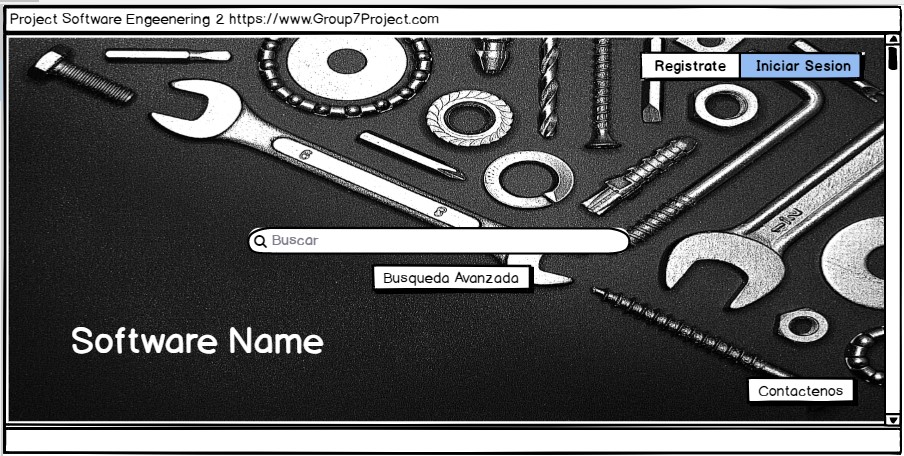
\includegraphics[scale = 0.4]{images/PaginaPrincipal.png}
    \caption{Pagina Principal}
    \label{F00}
\end{figure}{}


\begin{landscape}
\section{Modelo Entidad Relación}
    \begin{figure}[H]
        \centering
        
\includegraphics[scale = 0.5]{images/escudoUN.png}
        \caption{Descripción}
        \label{F01}
    \end{figure}{}
\end{landscape}


\section{Modelo de Base de Datos}

\section{Estimación de Costos}

% plantilla: copiar y pegar
\begin{table}[H]
    \centering
    \small{
    \begin{tabular}{R{6cm}L{6cm}}
        \textbf{Concepto}   &\textbf{Valor}\\
        \\
        \multicolumn{2}{c}{Holi \dotfill \$10'000.000} \\
        \multicolumn{2}{c}{Holi \dotfill \$10'000.000} \\
        \hline
        \multicolumn{2}{c}{\textbf{Total} \dotfill \$10'000.000} \\
    \end{tabular}
    \label{T03}}
\end{table}{}


\section{Análisis de riesgos}


\begin{table}[H]
    \centering
    \small{
    \begin{tabular}{|M{1cm}|M{3cm}|M{8cm}|}
        \hline
        \textbf{Valor}  &\textbf{Tipo}   &\textbf{Definición}\\
        \hline 
        \multirow{1}{1cm}{\centering 1}    
            & \multirow{1}{3cm}{\centering Técnico}
            & Criterio      \\
        \hline
        \multirow{1}{1cm}{\centering 2}
            & \multirow{1}{3cm}{\centering Organizacional}
            & Criterio      \\
        \hline
        \multirow{1}{1cm}{\centering 3}
            & \multirow{1}{3cm}{\centering Cronograma}
            & Criterio      \\
        \hline
        \multirow{1}{1cm}{\centering 4}
            & \multirow{1}{3cm}{\centering Externo}
            & Criterio      \\
        \hline
        \multirow{1}{1cm}{\centering 5}
            & \multirow{1}{3cm}{\centering Gerencial}
            & Criterio      \\
        \hline
    \end{tabular}
    \caption{Tipos de riesgo}
    \label{Riesgo}}
\end{table}{}


\begin{table}[H]
    \centering
    \small{
    \begin{tabular}{|M{1cm}|M{2cm}|M{8cm}|}
        \hline
        \textbf{Valor}   &\textbf{Significado}   &\textbf{Criterio}\\
        \hline 
        \multirow{1}{1cm}{\centering 1}    
            &\multirow{1}{2cm}{\centering Muy bajo}
            & Criterio      \\
        \hline
        \multirow{1}{1cm}{\centering 2}    
            &\multirow{1}{2cm}{\centering Bajo}
            & Criterio      \\
        \hline
        \multirow{1}{1cm}{\centering 3}    
            &\multirow{1}{2cm}{\centering Moderado}
            & Criterio      \\
        \hline
        \multirow{1}{1cm}{\centering 4}    
            &\multirow{1}{2cm}{\centering Alto}
            & Criterio      \\
        \hline
        \multirow{1}{1cm}{\centering 5}    
            &\multirow{1}{2cm}{\centering Muy alto}
            & Criterio      \\
        \hline
    \end{tabular}
    \caption{Niveles de Impacto}
    \label{Nimpacto}}
\end{table}{}

\begin{table}[H]
    \centering
    \small{
    \begin{tabular}{|M{3.5cm}|M{1cm}|M{1.5cm}|M{2.5cm}|M{4cm}|}
         \hline
            \textbf{Riesgo} & \textbf{Tipo} &\textbf{Impacto}
            & \textbf{Probabilidad} & \textbf{Plan de acción}\\
         \hline
         \multirow{1}{3cm}{\centering Ries}
             & \multirow{1}{1cm}{\centering 1}
             & \multirow{1}{1.5cm}{\centering 5}
             & \multirow{1}{2.5cm}{\centering 50\%}
             &  Descrip     \\
        \hline
         \multirow{1}{3cm}{\centering Ries}
             & \multirow{1}{1cm}{\centering 1}
             & \multirow{1}{1.5cm}{\centering 5}
             & \multirow{1}{2.5cm}{\centering 50\%}
             &  Descrip     \\
        \hline
         \multirow{1}{3cm}{\centering Ries}
             & \multirow{1}{1cm}{\centering 1}
             & \multirow{1}{1.5cm}{\centering 5}
             & \multirow{1}{2.5cm}{\centering 50\%}
             &  Descrip     \\
             
        \hline
         \multirow{1}{3cm}{\centering Ries}
             & \multirow{1}{1cm}{\centering 1}
             & \multirow{1}{1.5cm}{\centering 5}
             & \multirow{1}{2.5cm}{\centering 50\%}
             &  Descrip     \\
        \hline
         \multirow{1}{3cm}{\centering Ries}
             & \multirow{1}{1cm}{\centering 1}
             & \multirow{1}{1.5cm}{\centering 5}
             & \multirow{1}{2.5cm}{\centering 50\%}
             &  Descrip     \\
        \hline
         \multirow{1}{3cm}{\centering Ries}
             & \multirow{1}{1cm}{\centering 1}
             & \multirow{1}{1.5cm}{\centering 5}
             & \multirow{1}{2.5cm}{\centering 50\%}
             &  Descrip     \\
        \hline
         \multirow{1}{3cm}{\centering Ries}
             & \multirow{1}{1cm}{\centering 1}
             & \multirow{1}{1.5cm}{\centering 5}
             & \multirow{1}{2.5cm}{\centering 50\%}
             &  Descrip     \\
        \hline
    \end{tabular}
    \caption{Riesgos de desarrollo}
    \label{riesgos}}
\end{table}{}


\begin{thebibliography}{50}
\bibitem{00} Description. Disponible en: \url{https://github.com}

\end{thebibliography}{}

\end{document}{}
